\chapter{FPGA Design \& Implementation} 
% architecutr &design & impementation
\label{Chapter-FPGA-Implementation}

\section{Tools Used}
\subsection{Vitis Unified Software Platform}
The Vitis unified software platform\cite{Vitis_unified_software_platform} is a collection of tools, libraries and environments designed to ease the development of accelerated applications tailored for AMD Xilinx FPGA and Versal® ACAP hardware platforms. It includes graphical and command-line compilers, analyzers, and debuggers to build applications, analyze performance bottlenecks, and debug accelerated algorithms, developed in C, C++, or OpenCL APIs. Furthermore, it offers numerous advantages such as effortless application portability, complete simulation of hardware systems, and an open source runtime that handles host-device communication.
\begin{figure}[H]
    \centering
        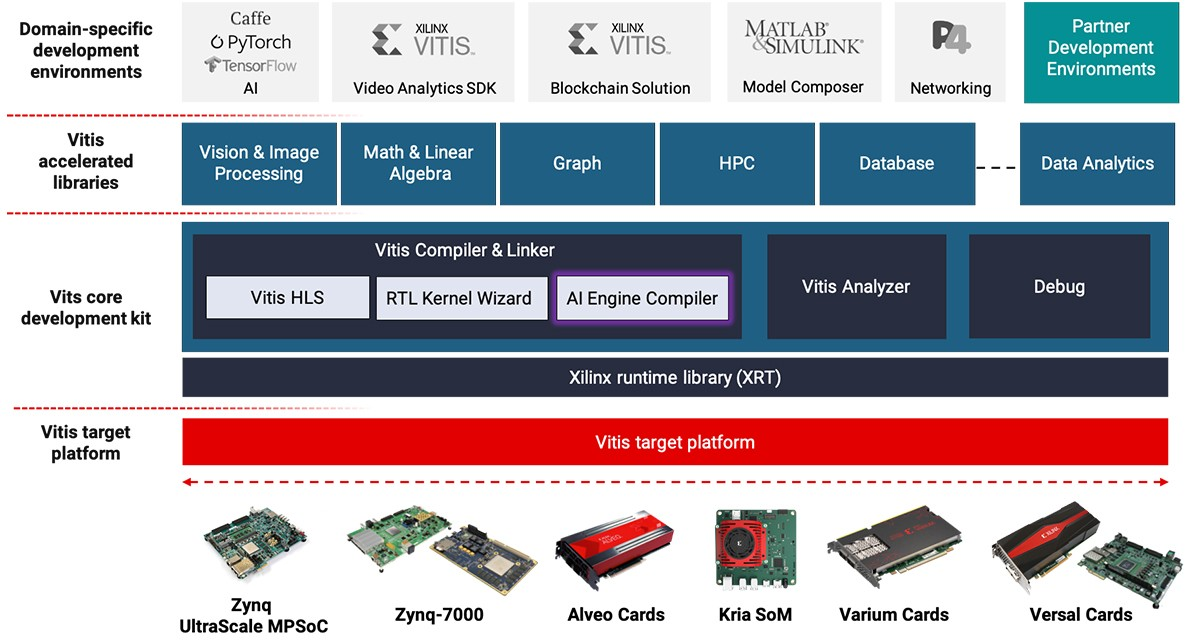
\includegraphics[width=1\textwidth]{Images/Platform/vitis.jpg}
        \decoRule
        \caption[Vitis]{Vitis overview: \href{https://www.xilinx.com/products/design-tools/vitis/vitis-platform.html\#overview}{URL}.}
        \label{fig:Vitis_overview}
\end{figure}

Vitis supports hardware acceleration kernels controlled by PS or x86 kernels. The Vitis application acceleration development flow provides a framework for developing and delivering FPGA-accelerated applications using standard programming languages for both software and hardware components. The kernels can be developed through traditional RTL, C/C++ with Vitis HLS, the Vitis model composer and the AI Engine compiler.
\begin{figure}[H]
    \centering
        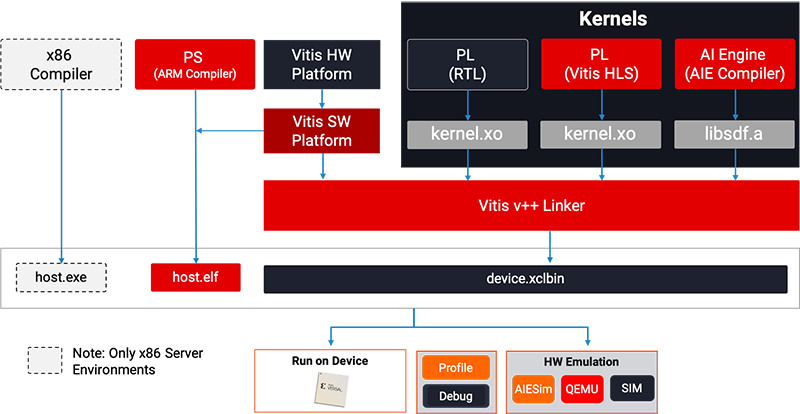
\includegraphics[width=1\textwidth]{Images/Platform/vitis_kernel.png}
        \decoRule
        \caption[Vitis]{Vitis kernel architecture: \href{https://www.xilinx.com/products/design-tools/vitis/vitis-platform.html\#development}{URL}.}
        \label{fig:Vitis_kernel_overview}
\end{figure}

\subsection{Xilinx Runtime library (XRT)}
The Xilinx Runtime library\cite{Xilinx_Runtime_Library} (XRT) facilitates communication between the application code (running on an embedded Arm or x86 host) and the accelerators deployed on the reconfigurable portion of PCIe interface-based AMD Xilinx accelerator cards, MPSoC-based embedded platforms, or ACAPs. It is flexible with modifiable libraries and drivers, enabling different levels of abstractions, from high-level Python bindings to low-level C++ APIs. These APIs are common across all platforms and eliminate the need to implement hardware communication layers from scratch. % what is XRT

A widely used alternative are the OpenCL libraries. TBy abstracting the underlying implementations of numerous APIs, including the XRT, they offer a standard interface for managing heterogeneous devices. As a result, they enable portability across multiple devices from various providers, albeit with increased complexity due to the extra layer of abstraction. As this work is not indented to transition to other devices, the XRT is preferred. % why I chose XRT over OpenCL

\begin{figure}[H]
    \centering
        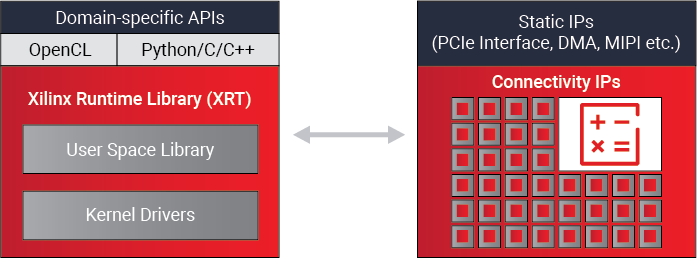
\includegraphics[width=1\textwidth]{Images/Platform/xrt.png}
        \decoRule
        \caption[Xilinx Runtime Library]{Xilinx Runtime Library overview: \href{https://www.xilinx.com/products/design-tools/vitis/xrt.html}{URL}.}
        \label{fig:XRT_overview}
\end{figure}

\subsection{Vitis High Level Synthesis (HLS)}
The Vitis HLS tool can synthesize a C/C++ function into RTL code for implementation in the programmable logic (PL) region of a Xilinx FPGA device. Its kernels can be easily integrated into a design utilizing OpenCL\cite{OpenCL} code. It provides support of complex data types, math functions and AXI4-Stream interfaces for data exchange between IPs in the PL and/or Processing Subsystem (PS).

HLS is an automated design process that takes an abstract behavioral specification of a digital system and generates a register-transfer level structure that implements the given behavior. The designer is working on a high abstraction level, while the tool takes care of mechanical RTL implementation tasks.

\begin{table}[H]
    \center
    \begin{tabular}{ | c | }
        \hline
        Designer's Responsibilities\\
        \hline
        Macro Architecture\\
        Design Intent\\
        Constrains\\
        \hline
        \multicolumn{1}{ c }{ } \\
        \multicolumn{1}{ c }{ } \\
        \multicolumn{1}{ c }{ } \\
        \multicolumn{1}{ c }{ } \\
    \end{tabular}
    \quad
    \begin{tabular}{ | c | }
        \hline
        HLS tool automation\\
        \hline
        FSM Generation\\
        Operation Scheduling\\
        Clock\\
        Register Pipelining\\
        Resource Sharing\\
        Timing\\
        Verification\\
        \hline
    \end{tabular}
    \caption[HLS responsibilities]{Distribution of work during HLS design.}
    \label{HLS responsibilities}
\end{table}

\section{FPGA Platforms}

\subsection{Xilinx Zynq UltraScale+ MPSoC}
The Zynq\textsuperscript{\textregistered} UltraScale+\texttrademark{} MPSoC is a family of Xilinx products that integrates a feature-rich 64-bit quad-core or dual-core Arm® Cortex®-A53 and dual-core Arm Cortex-R5F based processing system (PS) and Xilinx programmable logic (PL) UltraScale architecture in a single device. In addition, on-chip memory, multiport external memory interfaces, and a rich set of peripheral connectivity interfaces are included. \cite{Zynq_UltraScale_overview}

\subsection{ZCU102 Evaluation Board}
The ZCU102 Evaluation Board features a Zynq\textsuperscript{\textregistered} UltraScale+\texttrademark{} MPSoC with a quad-core Arm\textsuperscript{\textregistered} Cortex\textsuperscript{\textregistered}-A53, dual-core Cortex-R5F real-time processors, and a Mali\texttrademark{}-400 MP2 graphics processing unit based on Xilinx's 16nm FinFET+ programmable logic fabric. It supports all major peripherals and interfaces, enabling development for a wide range of applications. Furthermore, its high speed DDR4 memory interfaces, variety of communication interfaces and FMC expansion ports makes it ideal for rapid prototyping. 

\begin{figure}[H]
    \centering
        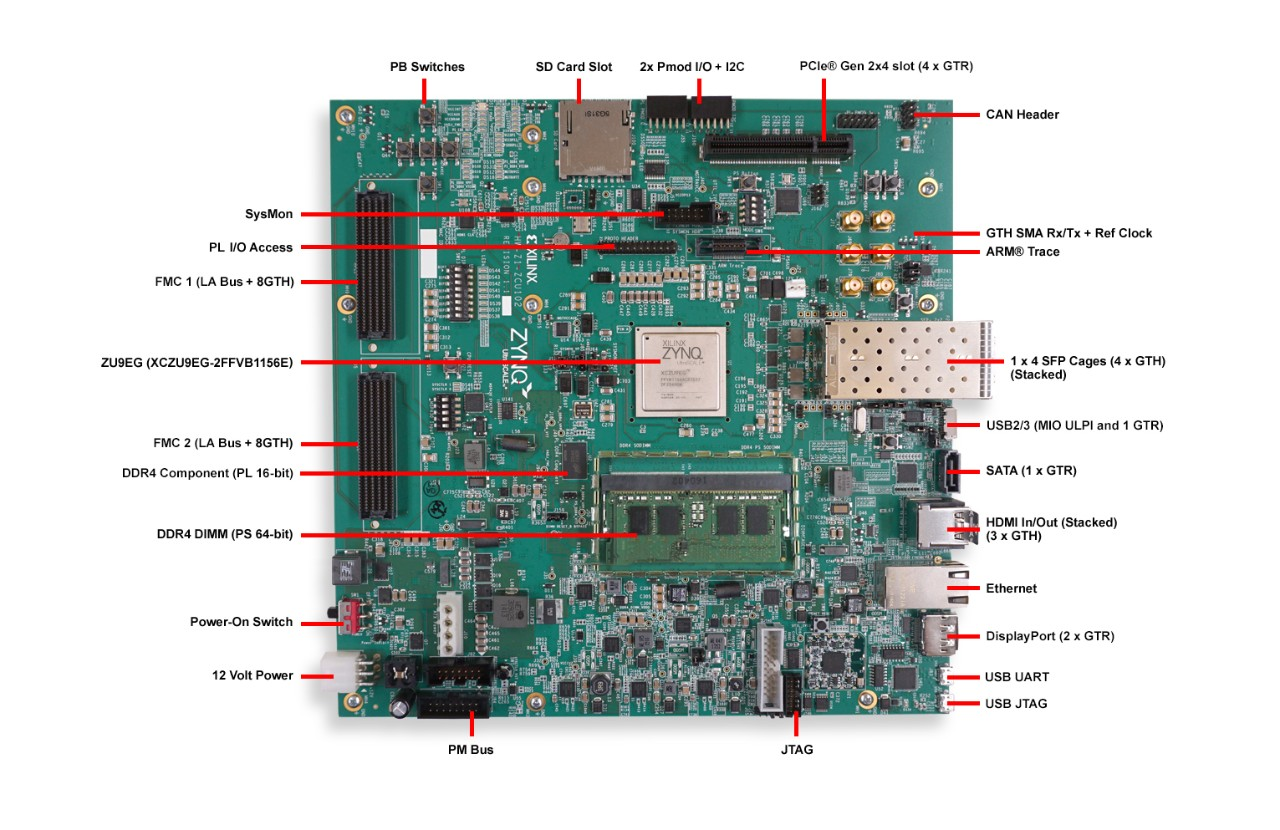
\includegraphics[width=1\textwidth]{Images/Hardware/zcu102.jpg}
        \decoRule
        \caption[ZCU102]{ZCU102 Features: \href{https://www.xilinx.com/products/boards-and-kits/ek-u1-zcu102-g.html\#information}{URL}.}
        \label{fig:ZCU102}
\end{figure}

Given that the thesis is based on an edge application, this platform seems to be an ideal fit for it. During the hardware design phase, the constrains and resource limitation were placed according to the specifications of this board. Nevertheless, transferring the final design to devices of similar families should require minimal effort.

\section{Preparing the CNN for Hardware}
In the preceding phase, TF with Python was utilized to implement all ANNs and training. As the Vitis Kernel Toolchain is aimed to C/C++ code, these implementations can not be synthesized to hardware by the aforementioned tools. As such, a simplified version of the most used CNN, the third in the model library, has been re-implemented with C++.

Migrating from TF to a hardware synthesizable CNN is a fairly challenging task riddled with pitfalls. This implementation is not optimized for hardware, but rather serves as a stepping stone between TF and synthesizable code. Certain practices are adopted to facilitate future transition to hardware targeted code:

\begin{itemize}[leftmargin=*]
    \item Implementation is modular and re-configurable. The code is build around template functions, each of which performs a specified task. Layers can effortlessly added, removed, or altered in size, shape and parameters.
    \item All data, whether input, output or internal, are produced and consumed serially and only once. This behavior is similar to the stream data format, which is widely utilized in hardware design.
    \item All feature maps, input gradients, variable gradients, and updated variables are logged and compared with those generated by the existing TF implementation. This approach not only evaluates functionality, but also produces test benches for future hardware implementation.
\end{itemize}

\begin{figure}[H]
    \centering
        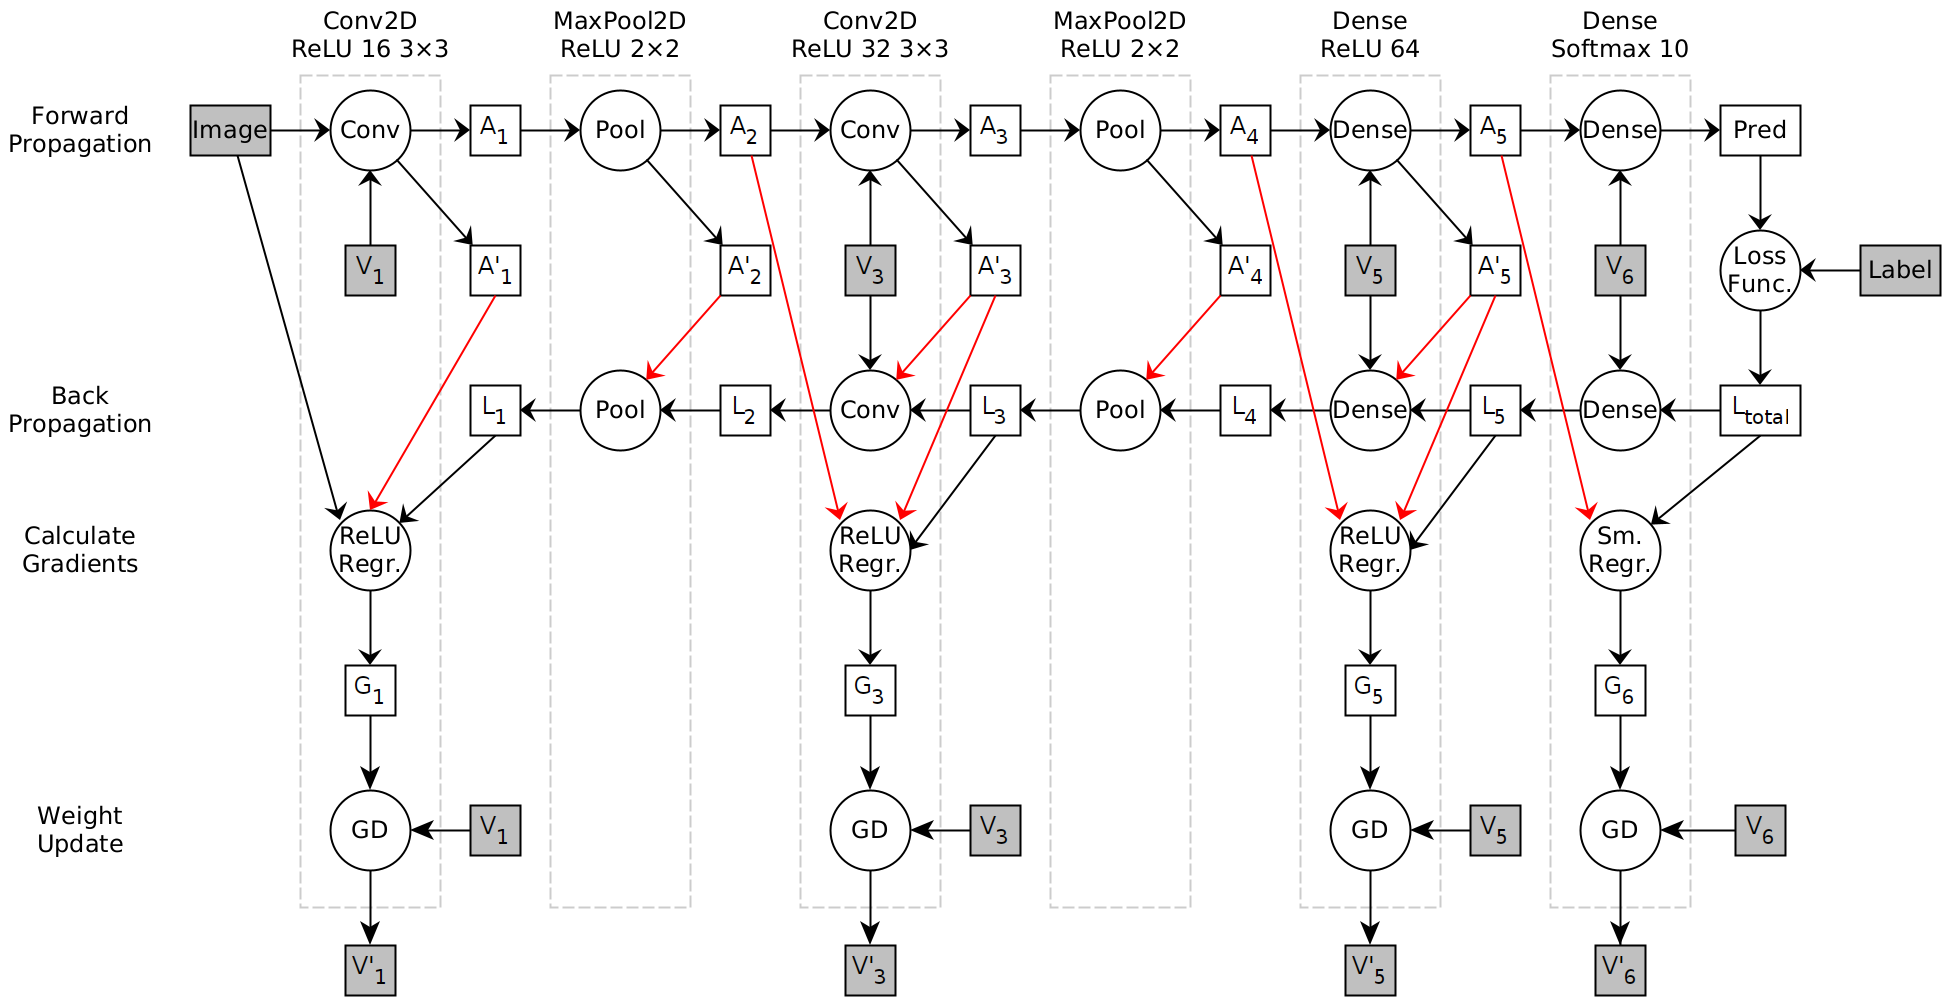
\includegraphics[width=1\textwidth]{Images/block_diagrams/dataflow_cnn_model.png}
        \decoRule
        \caption[CNN dataflow]{Dataflow diagram of the utilized CNN model.}
        \label{fig: CNN dataflow}
\end{figure}

Figure \ref{fig: CNN dataflow} depicts the basic structure of the implementation. Tasks are represented by cycles, whereas data are represented by squares. Inputs, labels, weights and any other data that must to be saved in memory have greyed-out squares. The majority of internal data are consumed immediately after being produced. Some of them, marked by red arrows, skip parts of the chain and must be temporally stored.

\section{Vitis HLS Hardware Implementation}
Even with the aforementioned techniques, adapting the code to be compatible with FPGAs is not a trivial task. To build an efficient implementation, resource usage, data access patterns, and other factors must be taken into account. All parts of the CNN are modified accordingly.

\subsection{2D Convolutional Layers}
Due to their non-serial data access patterns, multi-dimensional filter algorithms frequently conflict with FPGA design; 2-D convolution is no exception. At its core, it carries out some form of data averaging around a pixel, necessitating the access of nearby input values as seen in figure \ref{fig: convolution access pattern}. Additionally, when calculating the adjacent outputs, some inputs are accessed again.

\begin{figure}[H]
    \centering
        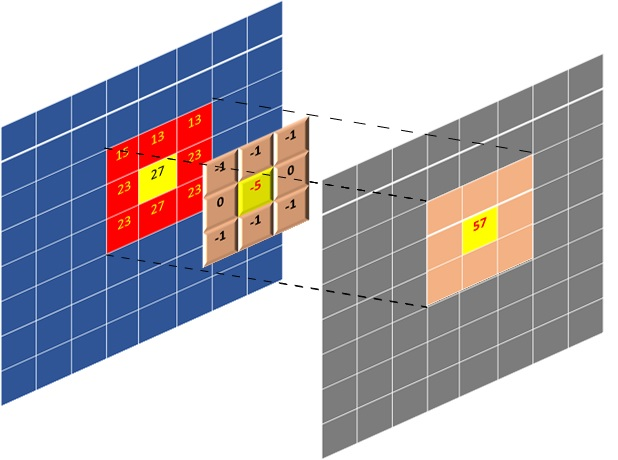
\includegraphics[width=1\textwidth]{Images/diagrams/convolution_access_pattern.jpg}
        \decoRule
        \caption[convolution access pattern]{Convolution access pattern: Input (Blue) pixels are accessed in a non-serial pattern.\href{https://github.com/Xilinx/Vitis-Tutorials/blob/2022.1/Hardware_Acceleration/Design_Tutorials/01-convolution-tutorial/lab1_app_introduction_performance_estimation.md}{URL} }
        \label{fig: convolution access pattern}
\end{figure}

In a CPU-focused implementation this would be a non issue, as data caching and pre-fetching can ensure that the majority of accesses will be cache hits. Implementing this on an FPGA would produce numerous small non-burst accesses on the global memory, resulting in unacceptable performance. Thus, a different approach is required.

A unique data mover, specifically designed for the given algorithm, has been developed to reduce the number of global memory accesses. Its key concept is to construct two-dimensional input windows that are the same size as the filters and then compute the dot product of those. Its main components are buffers that store lines of the input, and a sliding window on top of them.

\begin{figure}[H]
    \centering
        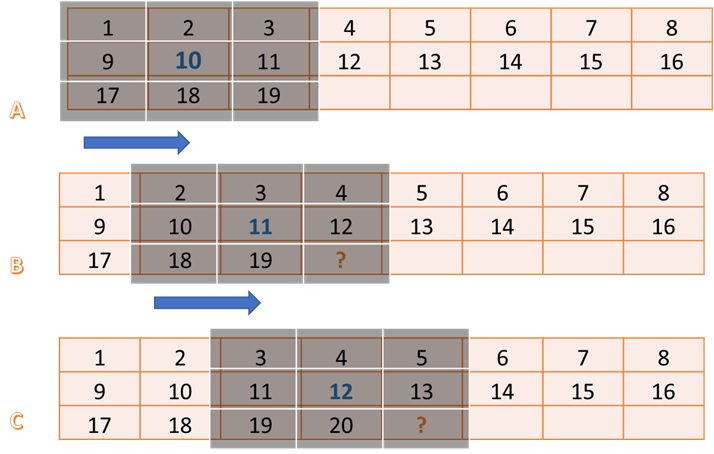
\includegraphics[width=1\textwidth]{Images/diagrams/line_buf_conv.jpg}
        \decoRule
        \caption[Line Buffers, Convolution]{Line Buffers: Sifting a 3x3 window. \href{https://github.com/Xilinx/Vitis-Tutorials/blob/2022.1/Hardware_Acceleration/Design_Tutorials/01-convolution-tutorial/lab2_conv_filter_kernel_design.md}{URL} }
        \label{fig: Line Buffers Convolution}
\end{figure}

Figure \ref{fig: Line Buffers Convolution} illustrates the operation of the line and window buffering scheme. A continuous stream of 3x3 windows is produced by sifting a window buffer over the top of the line buffers. Since the masked elements of the top line are already present in the window, only two line buffers are needed. Furthermore, only one new input pixel is required to produce a window, and thus an output pixel. Finally, zero padding is applied to maintain correct data with edge windows.

To complete the 2D convolution, a processing element is required. In the simplest scenario, a single channel input, the dot products between the windows and the filters are calculated and activated with the ReLU function. If there are additional input channels, the dot products are calculated in respect of each channel, which are aggregated and then activated to produce the feature map of the layer. This is done to allow computing of multiple channels in parallel, while using a data streaming paradigm.

Two output streams are produced, one float and one bool. The first one consists of the activations and is connected to the next layer. The second one indicates whether or not the kernels have activated the ReLU function. As only activated neurons convey their error backwards, this is necessary information for the back-propagation.

\begin{figure}[H]
    \centering
        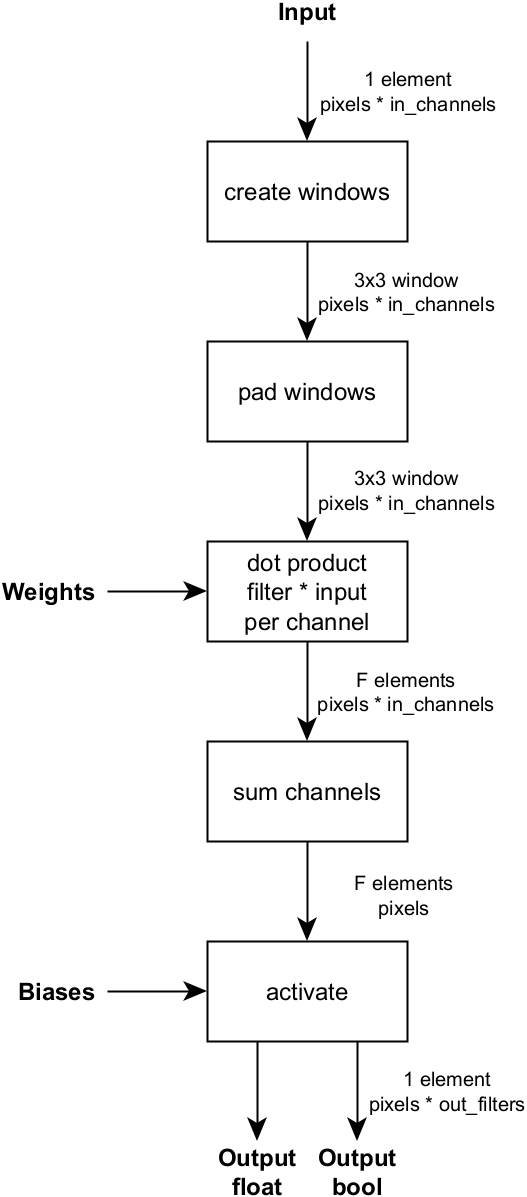
\includegraphics[width=0.406\textwidth]{Images/block_diagrams/conv2d_fp_mc.png}
        \decoRule
        \caption[Conv2D forward propagation block diagram]{Block diagram of the 2D convolution forward propagation. F is the number of filters. The data types of the internal streams with the total data passed are shown. }
        \label{fig: Conv2D forward propagation block diagram}
\end{figure}

The transformation from software to HLS hardware implementation is shown in the following pseudocode:
\begin{algorithm}[H]
    \caption[Conv2d Software implementation.]{2D Convolution: Software implementation.}
    \label{alg:Conv2d_SW}
    \begin{algorithmic}
        \Function {\textbf{SW Implementation}:}{}
            \For {$p$ in pixels}
                \For{$o$ in output channels}
                    \For{$i$ in input channels}
                        \State $out[p][o] \pluseq filter[o][i] * in[p][i]$
                    \EndFor
                    \State $out[p][o] = activate(out[p][o])$
                \EndFor
            \EndFor
        \EndFunction
    \end{algorithmic}
    $out[p][o]$, $filter[o][i]$ \& $in[p][i]$ have the dimensions of the filter. They can be multiple dimension arrays.
\end{algorithm}

\begin{algorithm}[H]
    \caption[Conv2d Software to HLS Transformation.]{2D Convolution: Software to HLS Hardware Transformation.}
    \label{alg:Conv2d_SW_to_HLS}
    \begin{algorithmic}
        \Function {\textbf{Step 1}: Transpose output channels dimension from time to space.}{}
            \For {$p$ in pixels}
                \For{$i$ in input channels}
                    \State $out[p][0] \pluseq filter[0][i] * in[p][i]$
                    \State $out[p][1] \pluseq filter[1][i] * in[p][i]$
                    \State $\ldots$ \Comment{output channel times}
                \EndFor
                \State $out[p][0] = activate(out[p][0])$
                \State $out[p][1] = activate(out[p][1])$
                \State $\ldots$ \Comment{output channel times}
            \EndFor
        \EndFunction
        
        \Function {\textbf{Step 2}: Split multiplications, additions \& activations in distinct functions.}{}
        \EndFunction
        \Function {Func A:}{}
            \For {$p$ in pixels}
                \For{$i$ in input channels}
                    \State $A[0] = filter[0][i] * in[p][i]$
                    \State $A[1] = filter[1][i] * in[p][i]$
                \State $\ldots$ \Comment{output channel times}
                    \State Write $(A[0], A[1], \cdots)$ to $streamA$
                \EndFor
            \EndFor
        \EndFunction
        \Function {Func B:}{}
            \For {$p$ in pixels}
                \For{$i$ in input channels}
                    \State Read $(A[0], A[1], \cdots)$ from $streamA$\
                    \State $B[0] \pluseq A[0]$
                    \State $B[1] \pluseq A[1]$
                    \State $\ldots$ \Comment{output channel times}
                \EndFor
                \State Write $(B[0], B[1], \cdots)$ to $streamB$
            \EndFor
        \EndFunction
        \Function {Func C:}{}
            \For {$p$ in pixels}
                \State Read $(B[0], B[1], \cdots)$ from $streamB$
                \State $out[p][0] = activate(B[0])$
                \State $out[p][1] = activate(B[1])$
                \State $\ldots$ \Comment{output channel times}
            \EndFor
        \EndFunction
    \end{algorithmic}
\end{algorithm}

\begin{algorithm}[H]
    \caption[Conv2d HLS implementation.]{2D Convolution: HLS implementation.}
    \label{alg:Conv2d HLS}
    \begin{algorithmic}
        \Function {\textbf{Step 3}: Make output channels dimension flexible between time \& space using HLS tools.}{}
        \EndFunction
        \Function {Func A:}{}
            \For {$p$ in pixels}
                \For{$i$ in input channels}
                    \State \#pragma HLS PIPELINE II=flexible
                    \For{$o$ in output channels} \Comment{If II=1 loop is flattened}
                        \State $A[o] = filter[o][i] * in[p][i]$
                    \EndFor
                    \State Write $(A[0], A[1], \cdots)$ to $streamA$
                \EndFor
            \EndFor
        \EndFunction
        \Function {Func B:}{}
            \For {$p$ in pixels}
                \For{$i$ in input channels}
                    \State \#pragma HLS PIPELINE II=flexible
                    \State Read $(A[0], A[1], \cdots)$ from $streamA$
                    \For{$o$ in output channels} \Comment{If II=1 loop is flattened}
                        \State $B[o] \pluseq A[o]$
                    \EndFor
                \EndFor
                \State Write $(B[0], B[1], \cdots)$ to $streamB$
            \EndFor
        \EndFunction
        \Function {Func C:}{}
            \For {$p$ in pixels}
                \State Read $(B[0], B[1], \cdots)$ from $streamB$
                \For{$o$ in output channels}
                    \State $out[p][o] = activate(B[o])$
                \EndFor
            \EndFor
        \EndFunction
    \end{algorithmic}
\end{algorithm}

The overall scheme is designed to maximize the data reuse providing maximum parallel data to the processing element, with minimum use of memory. Back propagation and gradient calculation follow the same logic with a few minor differences:

In back propagation, the input is the activated output gradients. To activate them, the system need to remember which neurons fired during forward propagation, as shown in figure \ref{fig: CNN dataflow}. Furthermore, the biases are not used, and the channel/filter dimensions are reversed. Finally the output are the gradients of the layer's input.

The processing element of the gradient calculation differs more. Instead of using the weights to calculate the outputs, the outputs are used to calculate the weight gradients. Furthermore, finding the bias gradients is trivial, as they are equal with the sum of all output gradients of their filter.

\begin{figure}[H]
    \centering
        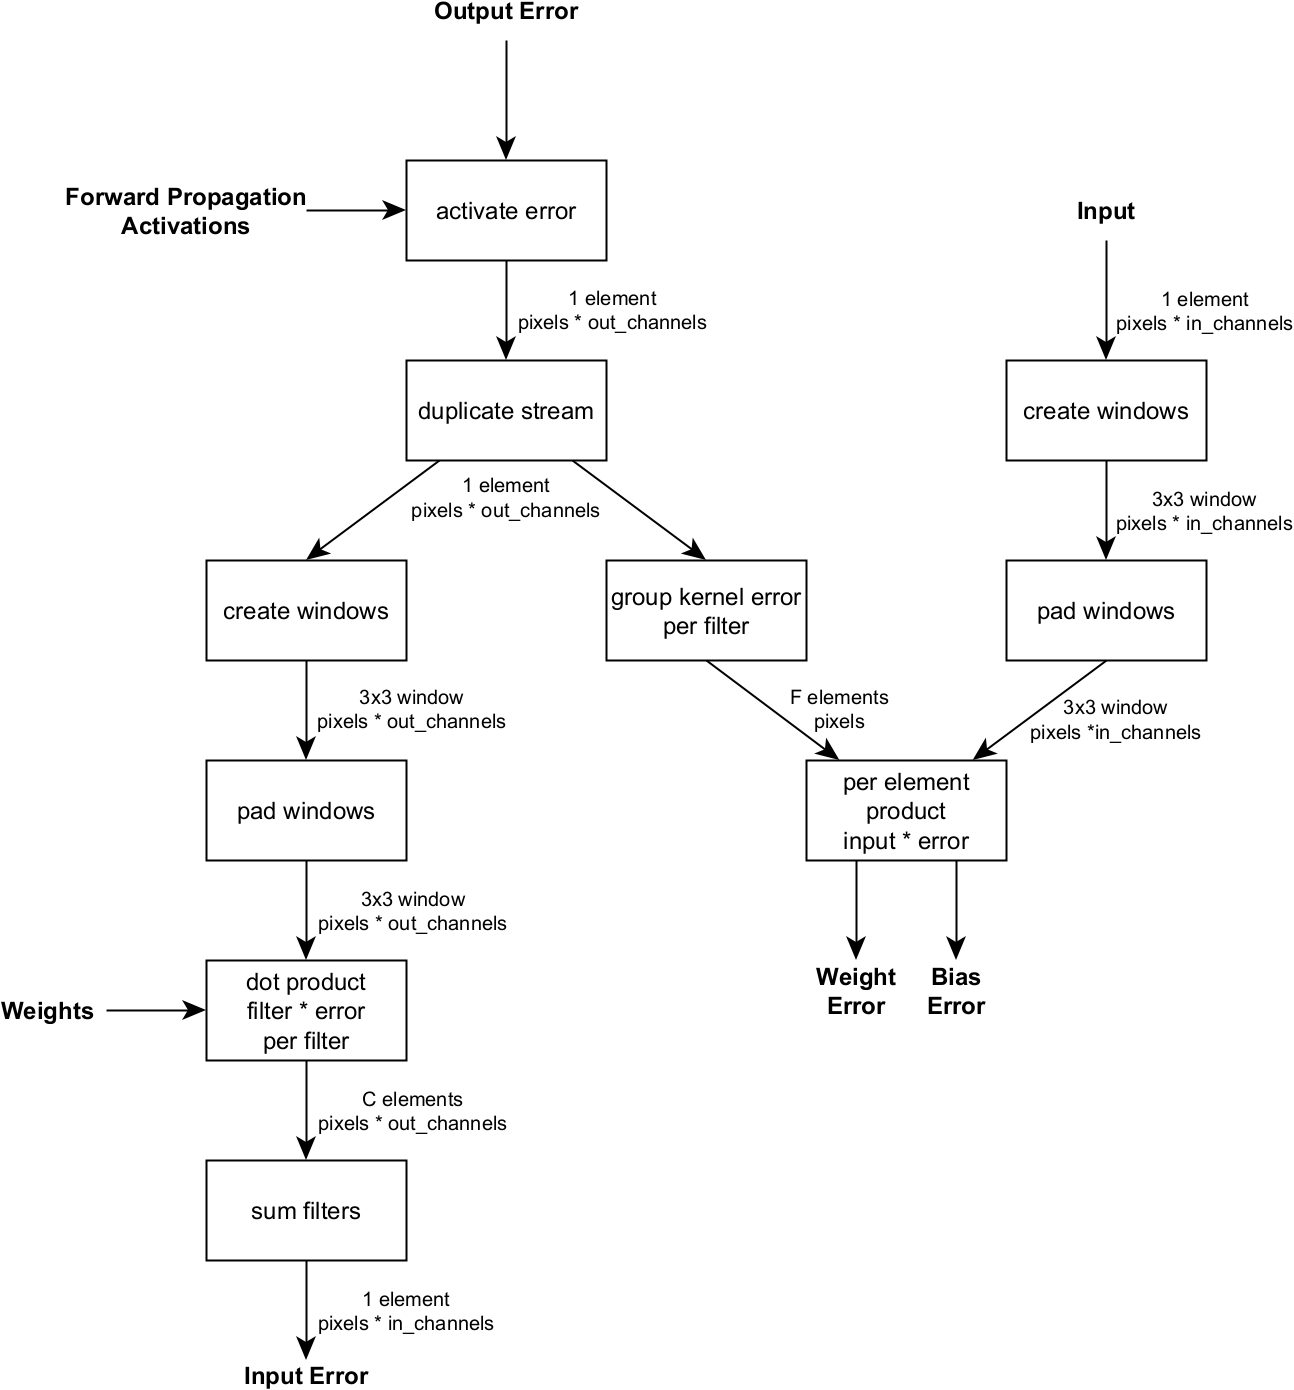
\includegraphics[width=1\textwidth]{Images/block_diagrams/conv2d_bp_cg_mc.png}
        \decoRule
        \caption[Conv2D back propagation block diagram]{Block diagram of the 2D convolution back propagation. F is the number of filters, C is the number of input channels. The data types of the internal streams with the total data passed are shown. }
        \label{fig: Conv2D back propagation block diagram}
\end{figure}

\subsection{2D Max-Pooling Layers}
The 2D Max-Pooling layers are implemented using the same logic as the 2D convolutional layers, albeit with a few major differences. First of all the window is 2x2 is size, and with a stride of 2. As a result, each window contains exclusive data, and an output can only be obtained with four inputs.

\begin{figure}[H]
    \centering
        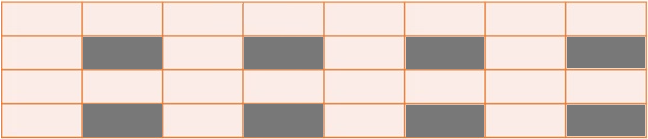
\includegraphics[width=1\textwidth]{Images/diagrams/line_buf_maxp.png}
        \decoRule
        \caption[Line Buffers, Max-Pool]{Line Buffers, Max-Pool: Grey pixels represent which inputs will trigger an output generation.}
        \label{fig: Line Buffers Max-Pool}
\end{figure}

Figure \ref{fig: Line Buffers Max-Pool} demonstrates the Max-Pool layer's uneven output generation, an unavoidable issue of any algorithm with stride greater than one. Following hardware does not operate while there are no data available, which is a problem in a FPGA design, as idle hardware indicates wasted hardware space. By raising the Iteration Interval (II) of the following hardware functions and properly calibrating the size of internal FIFO streams, the constant operation of the entire system is ensured.

The processing component of forward propagation is quite simple, as the output is the highest value in each window. It is important to note that the output's spatial dimensions are two times smaller than those of the input. Even more straightforward is back-propagation, in which the error back-propagates towards the maximum of each window. All other connections are assigned zero error gradients.

\subsection{Dense \& Softmax Layers}
The implementations of the dense and Softmax layers are simple and fairly similar. They are made up of two components: matrix multiplication of their inputs and weights and their respective activation function. In back-propagation and gradient calculation, the output error is activated before used as the input, with the input and variable gradients being the outputs.

The most crucial aspect of their design is ensuring that the hardware functions are constantly operating. To accomplish this, a streaming architecture, that reads and writes inputs and outputs serially and only once, is used. Important to note is that the Softmax activation requires all the inputs to be received before calculating any output, meaning that for an example back-propagation can not start until forward propagation is fully completed.

\subsection{Gradients Calculation Pipeline} % TODO: find better title
A major advantage of FPGA accelerators is that multiple hardware functions operate simultaneously, if the implemented algorithm allows. This holds true for most of the design. As an example, The first maxpool layer requires four inputs to generate the first output. These inputs have being generated by the first convolutional layer before a training data-point is fully loaded and processed. Thus the first two layers can operate simultaneously. % hardware function can operate simutanusly

On the other hand, the Softmax layer, which is the last step of the forward propagation, operates like a barrier. Due to the nature of the algorithm, to produce its feature map, all inputs must first be collected. As a result, for a single training data-point, the forward propagation must be completed before the back propagation begins. % softmax is a barrier

As such, the sequential semantics must be preserved, and the pipeline is implemented with a dataflow region that follows the control-driven task-level parallelism paradigm. This means that a subsequent function can start before the previous finishes and multiple functions can start and operate simultaneously. All tasks and channels are instantiated and connected explicitly. Furthermore, the inputs and outputs of the tasks are of stream type or stable memory arrays. % implementation

In this paradigm, the task with the highest latency typically determines the overall latency. Due to the existence of the Softmax barrier, for a single data input, forward propagation tasks can not operate simultaneously with tasks after it. As a result, the minimum overall latency equals the highest task latency before the barrier plus the highest task latency after it. % implementation barrier clash, overall latency

Figure \ref{fig: Gradients Calculation Pipeline Block Diagram} shows in detail the developed dataflow region that generates the weight and bias gradients. The heavy use of auxiliary data transformation functions, such as create windows and stream, is evident. These functions consume almost no hardware when synthesized, and add near zero latency. % auxiliary functions

Furthermore, several data streams skip hardware functions and layers. This could introduce stalls and ultimately deadlocks. To address this issue, hardware functions are implemented as free running pipelines $($FRPs$)$, when possible. Such implementations significantly reduce the possibility of a stall, by continuing to operate even when no input data are available or the output streams are full. % using frp and what they are

\begin{figure}[H]
    \centering
        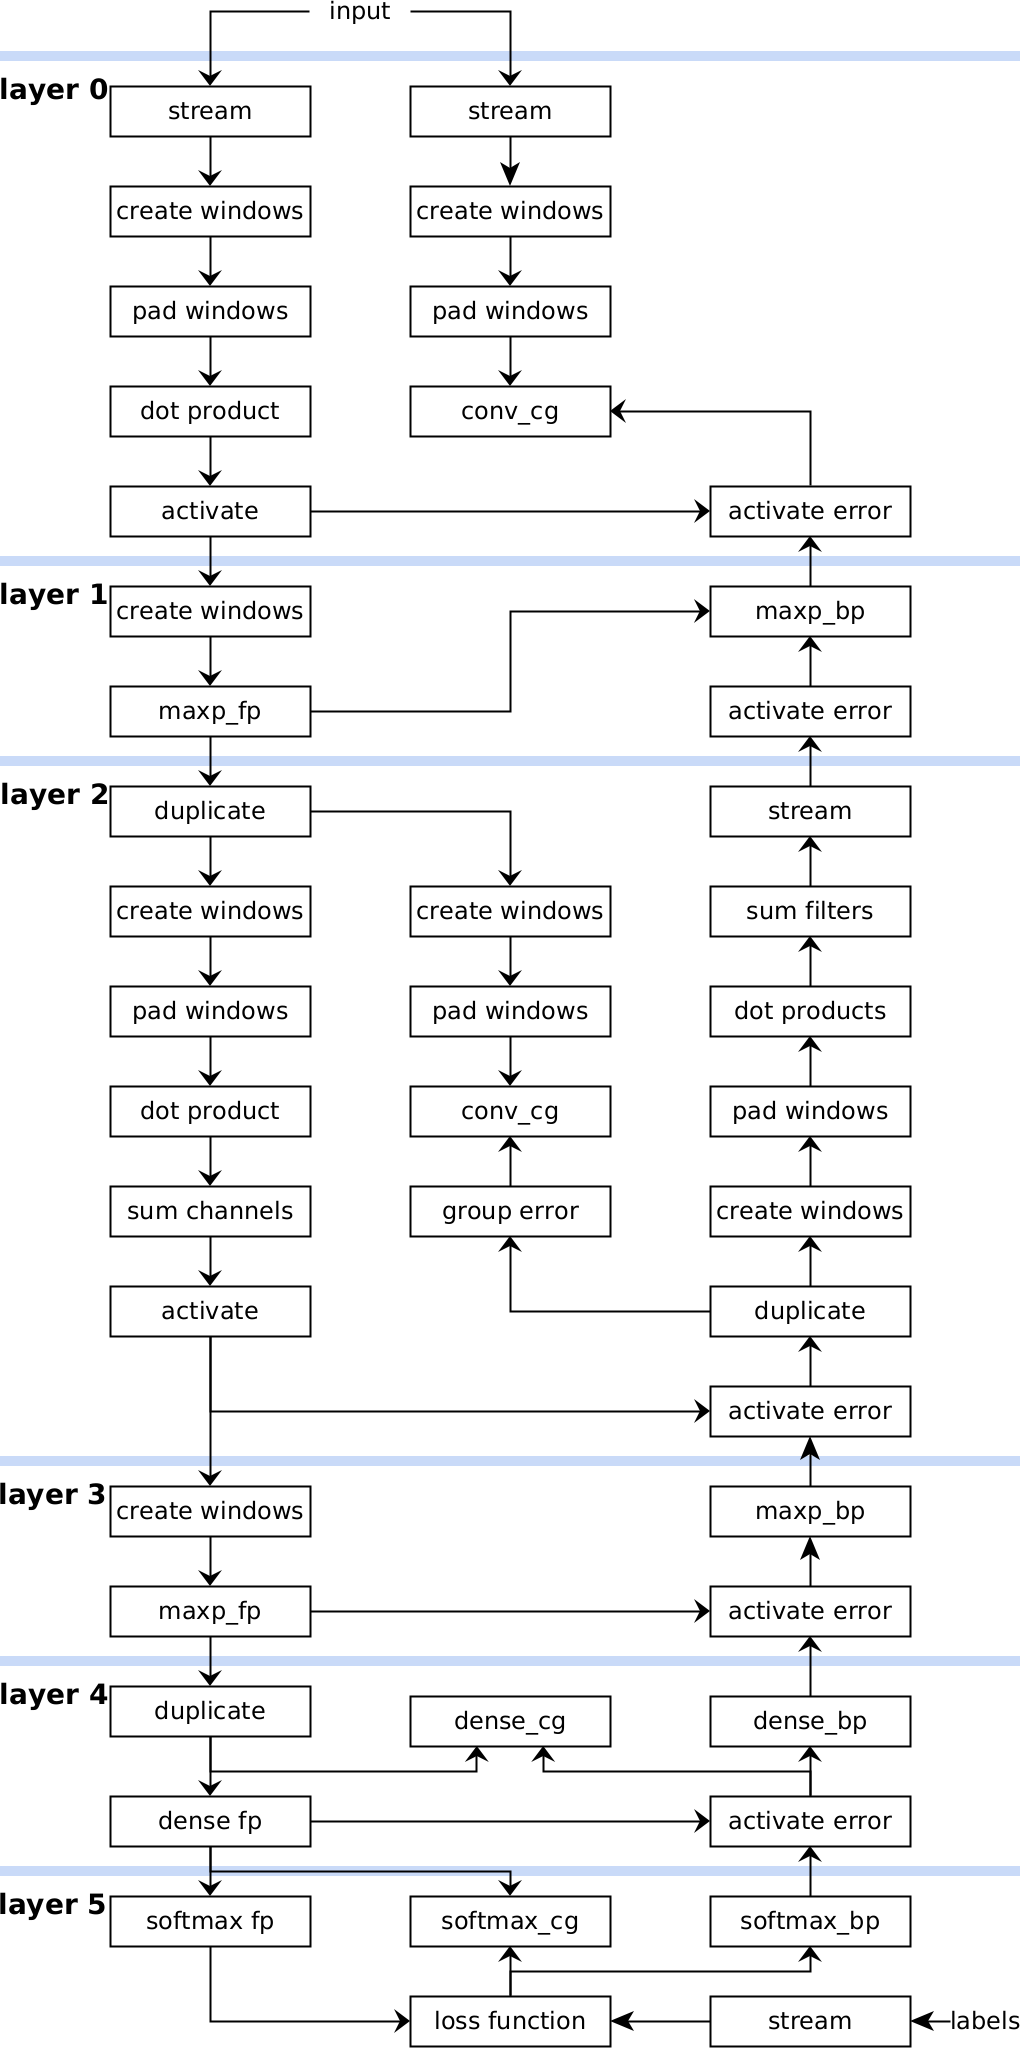
\includegraphics[height=0.95\textheight]{Images/block_diagrams/process_batch.png}
        \decoRule
        \caption[Gradients Calculation Pipeline Block Diagram]{Block diagram of the pipeline that generates the gradients. Inputs/Outpouts are not shown. Arrows represent data streams.}
        \label{fig: Gradients Calculation Pipeline Block Diagram}
\end{figure}
Using FRPs comes with multiple restrictions, a strict coding style is required, and MAXI ports are not supported. For hardware functions that read or write data from MAXI ports or can not adhere to other restrictions, flushable pipelines (FLPs) are used instead. They achieve the same goal as FRPs, but by instantiating multiple copies of the pipeline and executing them independently. As a result, the design is robust against any unpredictable stalls that MAXI ports may introduce. % FLPs and result

\subsection{Hardware Streams}
All communication between the hardware functions is facilitated with the stream implementation provided by the Vitis HLS library "hls\_stream.h". Hardware functions stall when an output stream is full, making the overall architecture inefficient. It is crucial to prevent this by determining the proper depth of the streams.

In most cases, this is trivial as they link sequential functions in a dataflow region where the consumer can instantly begin utilizing any data written by the producer. Then the major factor of the depth is the II of the connected functions. For most stream, a depth of two is sufficient.

More consideration is required about the streams that skip parts of the function chain. Due to the Softmax barrier, forward propagation of a sample is completed before its back propagation begins, thus all their data are produced before any of them is consumed. As such, their minimum depth is equal with the data produced by a single input sample.

To determine the ideal depths, an iterative optimization approach has typically been used. The Vitis HLS environment offers a variety of simulation tools that generate a number of useful statistics, such as the amount of clock cycles that each function stalls and whether or not a stream becomes full. Monitoring these when testing, enables calibrating the depths to ensure the stable flow of the pipeline, while not wasting hardware space in unnecessarily large streams.

\subsection{Batching Inputs}
As already explained, not all hardware functions can run concurrently for a single input sample. This issue is mitigated through batching input samples, where while an input runs through back-propagation, the next one is used in forward propagation. % description

\begin{figure}[H]
    \centering
        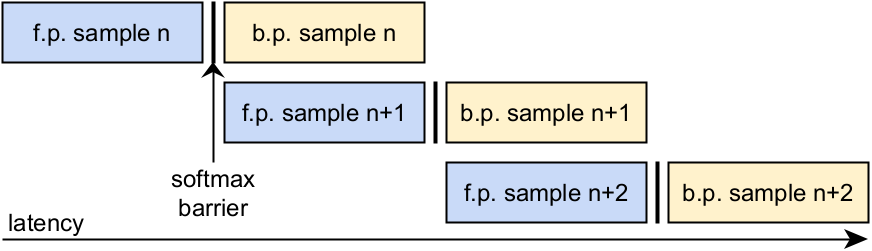
\includegraphics[width=\textwidth]{Images/diagrams/pipeline_under_batching.png}
        \decoRule
        \caption[Pipeline with batching latency]{ Latency of the pipeline under batching.}
        \label{fig: Batching Pipeline latency}
\end{figure}

With both sub-regions of the the pipeline having the same latency, the expected overall latency for a dataset without batching is defined as: % math
\begin{equation}
L_{dataset} = \sum^{samples}( L_{fp} + L_{bp} ) = 2 \cdot samples \cdot L_{fp/bp}
	\label{eqn: latency dataset no batching}
\end{equation}

With batching enabled, the latency of the dataset is transformed as:
\begin{equation}
    \begin{gathered}
        L_{dataset} = \sum^{\substack{batches\\ per\ dataset}}\sum^{\substack{samples\\ per\ batch}}( L_{fp/bp} + 1 ) =\\
        \frac{samples}{size_{batch}} \cdot size_{batch} \cdot ( L_{fp/bp} + 1 ) =\\
        samples \cdot ( L_{fp/bp} + 1 )
    \end{gathered}
	\label{eqn: latency dataset with batching}
\end{equation}

With Vitis HLS, implementing batching on each individual hardware function is quite trivial. Encapsulating their C++ definitions in a loop of the same size as the desired batch, is sufficient. % implementation

Further though must be given to the size of the streams connecting functions of the forward propagation with functions after the barrier. The producer functions will block until the consumer functions clear some space in the stream if the minimal depth is used as mentioned in the preceding section. Depending on the minimal latency between the producer and the consumer, this can be avoided by increasing the depth by 0.5 to 1 times.

\subsection{Updating Variables}
Based on the produced gradients, the variables of the ANN are updated in a second dataflow region. Due to the independence of all weights and gradients, the process is relatively straightforward. The basic gradient descend algorithm is used and the learning rate is supplied by the driver program. Thus, latency and hardware usage are the only criteria for the applied parallelism.

\subsection{Data Movement \& Storage}
Under the Vitis flow, AXI streams are unavailable for the ZCU102, thus memory mapping is used to transfer data from general memory to the PL and vice versa. These data are the input samples and labels, as well as the variables of the ANN. Appropriate data mover functions have been developed. % gmem <-> accel, which data

In Vitis HLS, arrays are implemented as continuous memory spaces with one or two ports, and only a limited amount of data can be read or written per cycle. To increase data accesses per cycle, the arrays are partitioned with the appropriate HLS directive \emph{ARRAY\_PARTITION}. The HLS tool splits the initial arrays to smaller ones, whose size and shape depend on the parameters of the corresponding directives. % array partition

The weights of the ANN are accessed in multiple functions of the first dataflow region and require special treatment. These arrays must be designated as shared using the directive \emph{STREAM} with the type parameter set to \emph{SHARED} in order for the design to be syntesizable. The tool then recognizes there are numerous consumers and multiplies the ports accordingly, without duplicating the array data. % shared arrays

For the weights of the second convolutional layer, this is insufficient. They are accessed by two functions with different access patterns. This issue can be resolved in two ways. The first one is satisfying both access patterns by increasing the partition factor and dimensions. This solution generate a huge amount of access ports, increasing hardware consumption unacceptably. More appropriate solution is creating two arrays with unique partitioning each. Albeit more memory is needed, the overall hardware usage is lower. % double arrays for layer 2 weights

When generating the gradients, the ANN's inputs, data and labels, are sent from global memory to the PL via AXI Master Adapter ports. In a dataflow region, each channel must have a single consumer, thus two ports are needed to propagate the input data to the two hardware functions that consume it. All ports are independent from one another by having their own dedicated bundles, thus enabling the simultaneous reading of all inputs. % dataflow inputs

The variable gradients are produced in the first dataflow region and consumed in the second, thus persistent saving in on-chip memory is necessary. The related arrays are not shared since their producers and consumers are in different regions, and can be implemented as streams or arrays, whichever is more convenient. % gradients

% \subsection{Minimizing Global Memory Accesses}
% bursting / port widening
% Rejected

\subsection{Top function}
To hold everything together, a top level function has been developed, whose signature operates as the API between PL and PS. Furthermore, it contains all the definitions of the memory structures, as well as the instantiations of the data movers and dataflow regions. Finally, to train on multiple batches, the dataflow regions are enclosed in a loop.

\begin{figure}[H] % TODO: remove the batch fetching
    \centering
        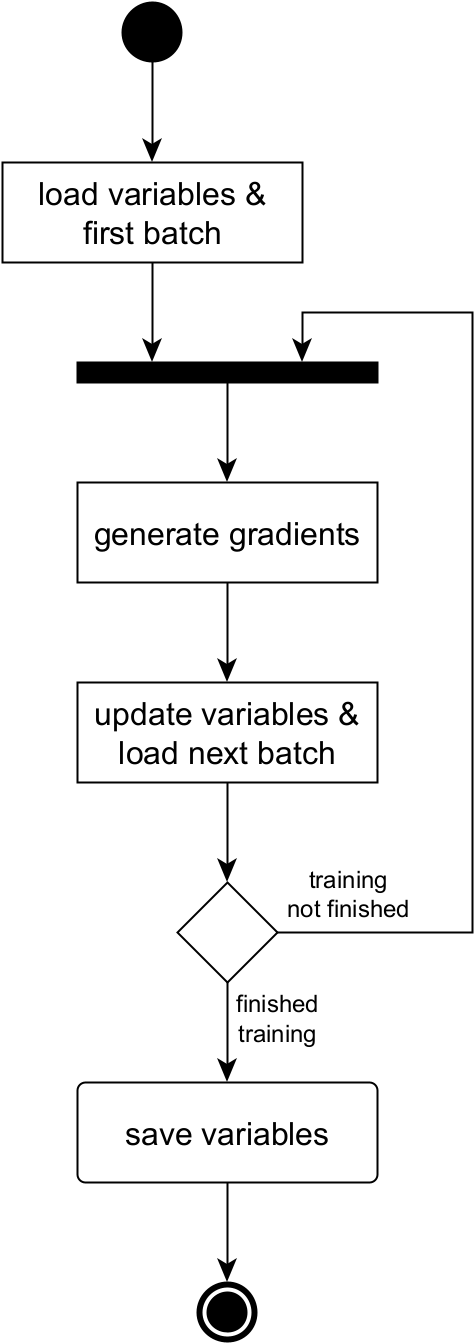
\includegraphics[height=0.5\textheight]{Images/block_diagrams/accel_top.png}
        \decoRule
        \caption[Top function]{Block diagram of the accelerator's top function.}
        \label{fig: top function}
\end{figure}

\section{Host Program}
The overall application uses Linux system calls, such as socket read and write. Thus a bare metal implementation is inadequate and a host program in the PS is required to drive the developed hardware design in the PL. This is achieved with the use of the XRT native C++ APIs \cite{XRT_Native_APIs}.

The flow of the driver code is as follows:
\begin{itemize}
    \item Open the device.
    \item Load the compiled and linked binary (XCLBIN) onto the device.
    \item Open the kernel loaded to the device with the XCLBIN.
    \item Create Buffer objects to transfer data to kernel inputs and outputs.
    \item Write data to the input buffers.
    \item Execute the kernel.
    \item Read data from the outputs buffers.
\end{itemize}
